\chapter{Medical Imaging}
\label{ch:rworks}

Medical imaging is a huge field of scope. The challenges are fascinating and so are the rewards. When we solve problems in medical imaging, we are literally serving humanity. Nowadays, medical imaging is widely different rather than even couple of years ago moreover than other areas of image processing. 

Mutually we are going to take a closer gaze at some of the basic techniques in medical imaging. It's an immense area so we going to pick a few particular specimens.

\section{Modalities}
To clarify in advance modalities in medical imaging can be considered as different types of images.

Each modality results from a different phenomenon of physics offers doctors (radiologists) an alternative view of the patient. Moreover each modality has it's risks, costs and benefits. All these factors have to be taken into account when choosing type of modality to be issued.

\subsection{X-Ray (X-RAY)}
In 1895, Wilhelm Roentgen explored rays which could pass through wood and human tissues. He called them \cite{Barker1996} 'x-rays' where 'x' was considered as a place-holder for the unknown.

X-Rays are a form of electromagnetic radiation in the same spectrum as visible light and radio waves. Like light, x-rays can be considered as a energy of an x-ray photon. To make x-rays, it can be fired high-energy electrons into matter. In medical-imaging applications, x-rays are sent into tissue. 

Jointly x-rays interactions with matter it can be considered 3 common cases:
\begin{itemize}
    \item Photoelectric Effect
    \newline This effect is the principal effect that makes x-ray useful.
    \item Compton Interaction
    \newline Because of tissues tend to have little variations, Compton Interaction does not give precise information in terms of what is inside the body. 
    \item Rayleigh (Coherent) Scattering
    \newline Upon interacting with the attenuating medium, the photon does not have enough energy to liberate the electron from its bound state.
\end{itemize}

\subsection{Computed Tomography (CT)}
In simplified terms, the idea of computed tomography is to resolve a single -- or a few slices -- slice of an object using many x-ray projections. As the gantry rotates, the scanner collects a 1D x-ray at each angle.

CT machine produces images projection which aim to be reconstructed into a 3D volume, which is a scalar field or set of voxels. 

\subsubsection{Contrast Agents}
As one of additional practices approaching CT for retrieving human body information, frequently substances can be introduced to the body to add the contrast, what is named as contrast agents. Often agents may be essentially useful for visualising of observations.          

\subsubsection{Motion Artifacts}
Usually it takes a few seconds to obtain one bit of CT data. The tidiness of the observations depends on whether the patient moved during the acquisition. If so, the resulting transformation will be inconsistent and the reconstructed image will contain errors. But, if the patient's motions are known, meaning a lot of artifacts can be corrected during the reconstruction. On top of it the few automatic methods can be applied to dare to sharpen the image by guessing the motions.

\subsection{Positron Emission Tomography (PET)}
Issuing PET technique we can consider the radiation traverse back and forth within the body (before issuing it is injected a small amount of positron-emitting radioisotope radiopharmacon, e.g.: FDG into patient body). PET detects counts and standard uptake value (SUV). Both CT and PET are super prompt and roughly take 4-5 minutes for acquisition.  
By nature the behaviour of different patients vary but the presence of willful and not willful movements made analyzing of body within its scanning more complicated, meaning the patient motions can cause the records inaccuracies. 

The list of images modalities and corresponding methods varies a lot strictly depending of the use case.
Below it is denoted few more popular directions:
\begin{itemize}
    \item MEG - Magneto Encephalography
    \item EEG -  Electro Encephalography
    \item OCT -  Optical Coherence Tomography
    \item SPECT -  Single-Photon Emission Computed Tomography
\end{itemize}

\section{Image Segmentation}
In terms of medical imaging, segmentation is the process of classifying pixels into groups which corresponds to the same tissue type. Segmentation has many uses cases like a 'measure volume of an organ', 'render a 3D view of an organ', 'surface-based registration' and many others. Further we will descry types of segmentation. 

\subsection{Thresholding}
The simplest method for classifying pixels based on solely on their intensity values. In thresholding we choose upper and lower bound and select pixels in predefined range.
The problem within simple thresholding is that it does not take into consideration any spatial information, meaning each pixel is evaluated no matter where it is located.    

\subsection{Region Growing}
Unlike basic thresholding, region growing -- which is iterative method -- starts with the small set of seed pixels and grow out from them.

The method functionality can be easily represented within any basic draw editor. To do that we will draw empty grid rectangle and afterwards select interested regions and apply function named 'flat fill' with chosen color. As a result it can be noticed the naive functionality handled the problem of tricking-out the selected regions by chosen color. This is so called region growing thresholding.    

\begin{figure}[h]
    \centering
    \begin{minipage}[b]{0.4\textwidth}
    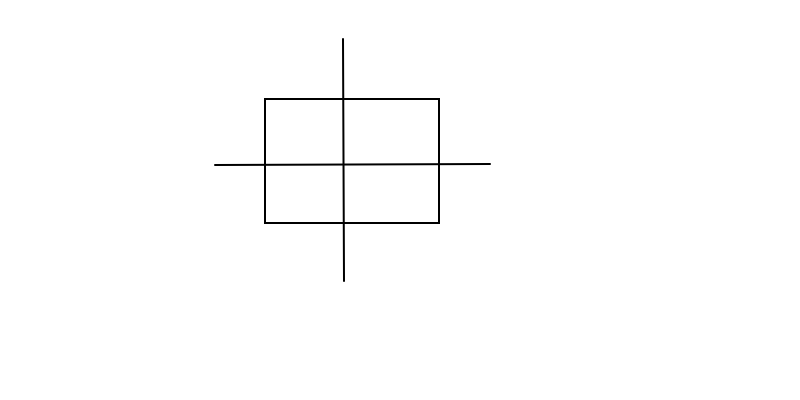
\includegraphics[width=\textwidth]{images/grow_region_0.png}
    \caption{Empty grid rectangle.}
    \end{minipage}
    \hfill
    \begin{minipage}[b]{0.4\textwidth}
    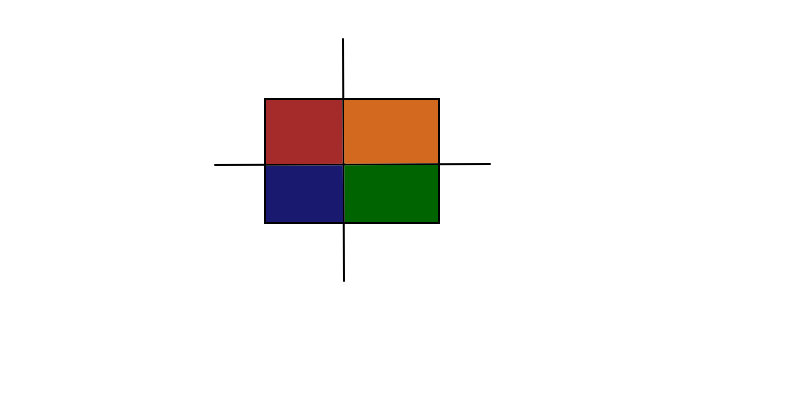
\includegraphics[width=\textwidth]{images/grow_region_1.png}
    \caption{Filled grid rectangle.}
    \end{minipage}
\end{figure}

Now, let us see how it is done from code base perspective.
\begin{lstlisting}
do
  for each pixel in the set
    for each of it's neighbours not in the set
      if the intensity falls between the thresholds
        add it to the set
      endif
    next neighbour
  next pixel
until no pixel were added in the last pass   
\end{lstlisting}

\newcolumntype{C}[1]{>{\centering\let\newline\\\arraybackslash\hspace{0pt}}m{#1}}
\newcolumntype{L}[1]{>{\raggedright\let\newline\\\arraybackslash\hspace{0pt}}m{#1}}

Example: There is set of pixels $4x4$ which should be colored. The cells which denoted by red color is already tricking-out. The task is fill rest with red color based on defined thresholding range.       

\begin{tabular}{C{7cm}  L{7cm}}
    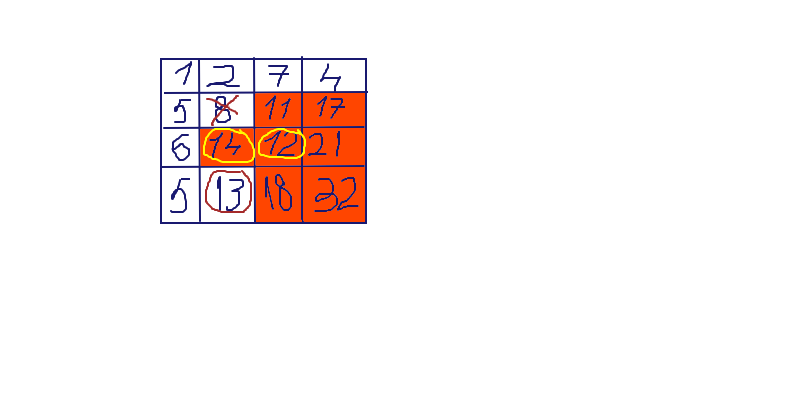
\includegraphics[width=12cm]{images/grow_region_3.png} & Thresholds: include a pixel if $10 \leq intensity \leq 100$ \newline 
    \begin{lstlisting}
    Looking at 14 ...
    up: 8 -> exclude (not in range)
    right: 12 -> skip (already in the set)
    down: 13 -> include as a new entry
    left: 6 -> exclude (not in range)
    \end{lstlisting}
\end{tabular}

Exactly the same way growing region thresholding method may be applied for medical images of different image modalities.
\begin{figure}[h]
    \centering 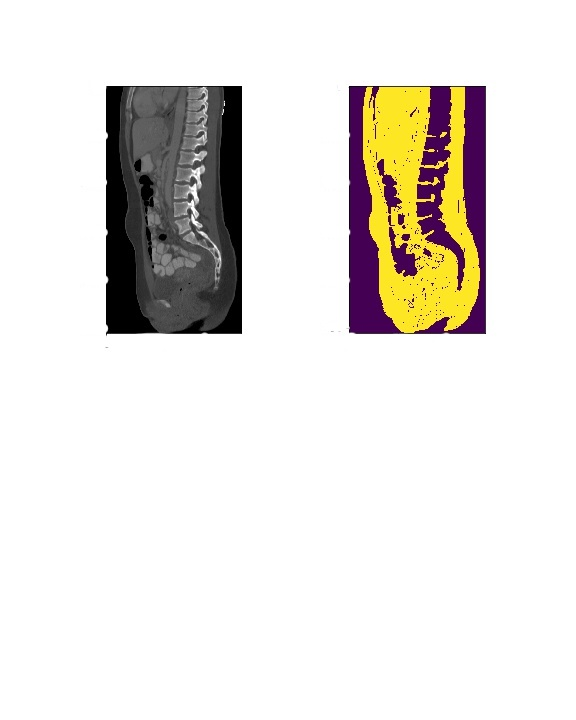
\includegraphics[width=8cm]{images/ct-spine-grow-region-segmented.jpg}
    \vspace*{-30mm} \caption {Original CT spine vs Segmented CT spine with Grow Region thresholding.}
\end{figure}    

There is a huge potential room for improvements making the method more sophisticated by coming up with different conditions for inclusion/exclusion of pixels.

\subsubsection{k-Means Clustering}
k-Means algorithm is very simple clustering method whereas usually the data set is represented as the a scatter plot in some feature space.

For instance, a pixel could be represented by 3 dimensional feature space, where feature space is defined by retrieving from the image following pixel-wise features:
\begin{itemize}
    \item Intensity
    \item Gradient magnitude
    \item Laplacian
\end{itemize}

First let us clarify the target results we are looking for by considering the very trivial task.
Assume, there is colorful triangle which should be clustered and represented in some feature space. Afterwards we can clearly see 3 different colors which denotes 3 clusters/groups.

\begin{figure}[h]
    \centering
    \begin{minipage}[b]{0.4\textwidth}
    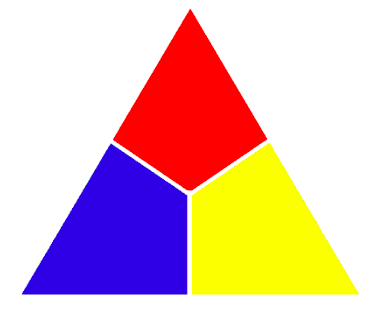
\includegraphics[width=\textwidth]{images/k_mean_triangle.png}
    \caption{Colorful triangle.}
    \end{minipage}
    \hfill
    \begin{minipage}[b]{0.4\textwidth}
    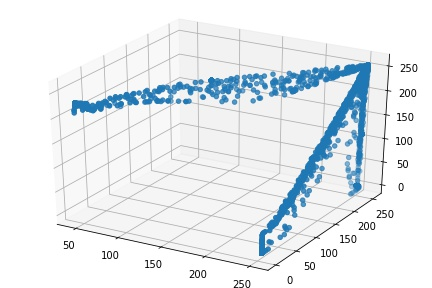
\includegraphics[width=\textwidth]{images/k_mean_triangle_clustered.jpg}
    \caption{Feature space representation.}
    \end{minipage}
\end{figure}


As for now, imagine, the user specified k the number of clusters, meaning how many different tissue types are in the image.
Hence, the algorithm may be defined as:
\begin{lstlisting}
1. (randomly) choose k regressors as prototype
2. assign each scatter point ('feature vector') to it's nearest regressor
3. recalculate new prototypes (the mean of it's members)
4. if the prototypes changed significantly -> go to the step 2 
\end{lstlisting}
To demonstrate the method we are going to proceed with the same ct spine scan data which had used for region growing thresholding. As for regressors number (clusters number) we will choose $k=3$.  

\newpage
\begin{figure}[h]
    \centering 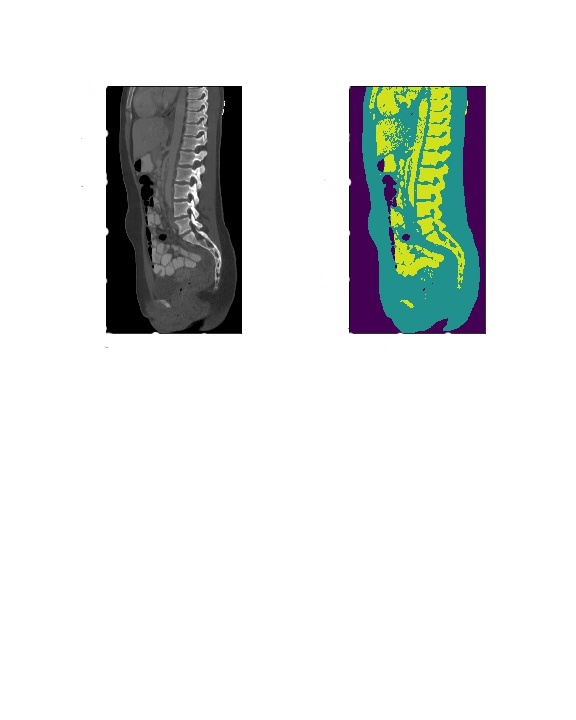
\includegraphics[width=8cm]{images/ct-spine-k-means-segmented.jpg}
    \vspace*{-40mm} \caption {Original CT spine vs Segmented CT spine with k-Means algorithm.}
\end{figure}    

As we can see, clustering is a really nice way for image segmentation, because you get to see the joint intensity of scatter plot (feature space) as well as different representations of clusters.  

There many more advanced segmentation techniques but before proceed further it worth briefly to discuss 2 more methods. We aim to shortly familiarize ourselves within their definitions and not dive to deep into details.      
\subsection{Snakes}
Shortly defined, it is active contour which is like a deformable boundary on an image designed to converge to an anatomical boundary of some sort. Deformable boundary is often represented by a number of nodes and vertices.  
The deformable boundary is often represented by a number of nodes and vertices.  

\subsection{Level Sets}
The level set method is a different way to formulate the active contour idea. Instead of explicitly modelling the curve the curve is implicitly modelled as a zero level set of a higher-dimension function. To model a curve in $\mathbf{R^n}$ we use an embedding function $\mathbf{R^n} \to \mathbf{R}$.     

